\section{Introduction}
\label{sec:intro}
Nowadays, advent of consumer friendly and affordable depth-cameras such as Kinect are commercially employed in many applications such as robotics and virtual reality.
%
Understanding and interpreting raw data provided by depth-cameras has drawn many attentions of researchers.
%
Whilst semantic segmentation as a fundamental part for understanding these raw data develops rapidly.
%
In the field of semantic segmentation, indoor scene parsing is a challenging problem due to cluttered backgrounds, a wide rang of scenes, object occlusions and various illumination.


In recent years, a great deal of studies have been conducted can be divided into three groups.
%
One group conducted semantic segmentation from single RGB image.
%
Another one attempted to add auxiliary information from depth for better segmentation.
%
The last one is multi-task learning which learns semantic segmentation with other tasks at the same time.


{\bf Semantic Segmentation from Single Image.}
%
Fully convolutional networks (FCN) is a milstone-like work for pixel-wise segmentation that converted the existing CNN constructed for classification to semantic segmentation.
%
To overcome the limitations of FCN that the network limited by a pre-defined fixed-size receptive field and always lost the detailed structures of objects, Noh \emph{et al.} \cite{Noh2015} proposed a novel deconvolution algorithm. 
%
Bayesian SegNet \cite{Kendall2015} performed visual scene understanding with a measure of model uncertainty to produce a probabilistic segmentation result.
%
To capture semantic correlations between neighboring patches and expoit the
patch-patch contextual information, Lin \emph{et al.} \cite{Lin2016} formulated conditional random fields (CRFs) with CNN-based pairwise potential function. 
%
For generating fine prediction, Lin \emph{et al.} \cite{Lin2017} proposed a multi-path refinement network that effectively exploits multi-level features to refine the prediction step by step.


{\bf Semantic Segmentation with Depth.}
%
Using extracted features from RGB images and depth images, Gupta \emph{et al.} \cite{Gupta2014} implemented an integrated system for scene understanding.
%
 A novel long short-term memorized context fusion (LSTM-CF) model is propposed by Li \emph{et al.} \cite{Li2016} to fuse contextual information from multiple sources such as RGB images and depth data.
% 
Cheng \emph{et al.} \cite{Cheng2017} rethought the relationship between RGB images and depth, and proposed a locality-sensitive deconvolution network to refine the boundary of segmentation result as well as a gated fusion layer to combine features of two modes.
%
Park \emph{et al.} \cite{Park2017} worked on how to fuse the multi-level RGB-D CNN features.
%
Therefore, they proposed a multi-modal feature fusion blocks and added it to RefineNet \cite{Lin2017}.


{\bf Multi-task Learning.} 
%
Eigen and Fergus \cite{Eigen2015} addressed three different tasks such as depth prediction, surface normal estimation, and semantic labeling using a single multiscale convolutional netwrok architecture. 
%
Prediction-and-distillationn network (PAD-Net) is another work\cite{Xu2018} which predicts a set of intermediate tasks including depth, surface normal, semantic and contour estimation, and then using the predictions from these tasks as multi-modal disitillation modules' inputs for final two tasks.  
%
A novel joint Task-Recursive Learning (TRL) \cite{Zhang2018} framework for semantic segmentation and depth estimation was proposed by Zhang. 
%
In TRL, two tasks are alternately processed in the decoder to imporve each other.
% 
Jiao \emph{et al.} \cite{Jiao2018} presented an attention-driven loss for network supervision and a synergy network to learn the information sharing strategies. 
%
By combining two tasks as well as proposed attention-driven loss, the performance of depth estimation and semantic segmentation are mutuallty improved.

\begin{figure*}[htbp]
	\centering
	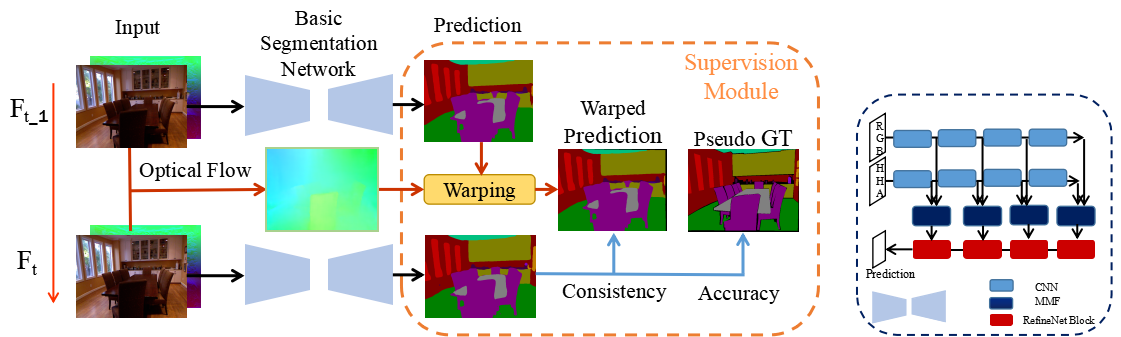
\includegraphics[scale=0.6]{figure/Pipeline.png}
	\caption{The overall architecture of our video-based semantic segmentation network. It mainly consists of three parts: 1) a basic segmentation model, which generates prediction of current frame 2) intermediate optical flow warpped part. We warp the previous prediction depend on optical flow 3) supervision module. Two supervisory items constitute our supervision module.}
	\label{fig:Pipeline}
\end{figure*}

Though above approaches provide a lot of novel ideas to improve the accuracy, the nature of data itself is ignored. 
%
Most of them do experiments on dense-annotated data sets, but there are many non-annotated images that have not been used.
%
It caused a huge waste of data.
%
In order to take full use of non-annotated images, in this paper, we propose two simple but effective ways. 
%
One is propagating labels from annotated frame to neighbouring non-aonnotated frames that generates many good quality and mixed noise pseudo ground truth (PGT) for network training. 
%
Compared to common data augmentation operations, it increases the diversity of training data.
%
The other is proposing a video-based semantic segmentation network with a temporal consistency constraint between frames. 
%
Due to most approaches being trained on image data set, jumping predictions often occur even in continuous frames of a video. 
%
As shown in Figure *.
%
It means that the network can not handle the problem of small perspective transformation well.
%
And the consistency of prediction results in time dimension could not be well maintained.
%
The rest of this paper is organized as follows.
% 
Our methodology will be introduced firstly.
%
Then, we will report the extensive experimental results as well as analyses. 
%
Finally we will draw a conclusion and propose our future work.
